\documentclass{standalone}
\usepackage{tikz}
\usetikzlibrary{patterns, positioning}
\usepackage[sfdefault]{ClearSans} %% option 'sfdefault' activates Clear Sans as the default text font
\usepackage[T1]{fontenc}

\begin{document}
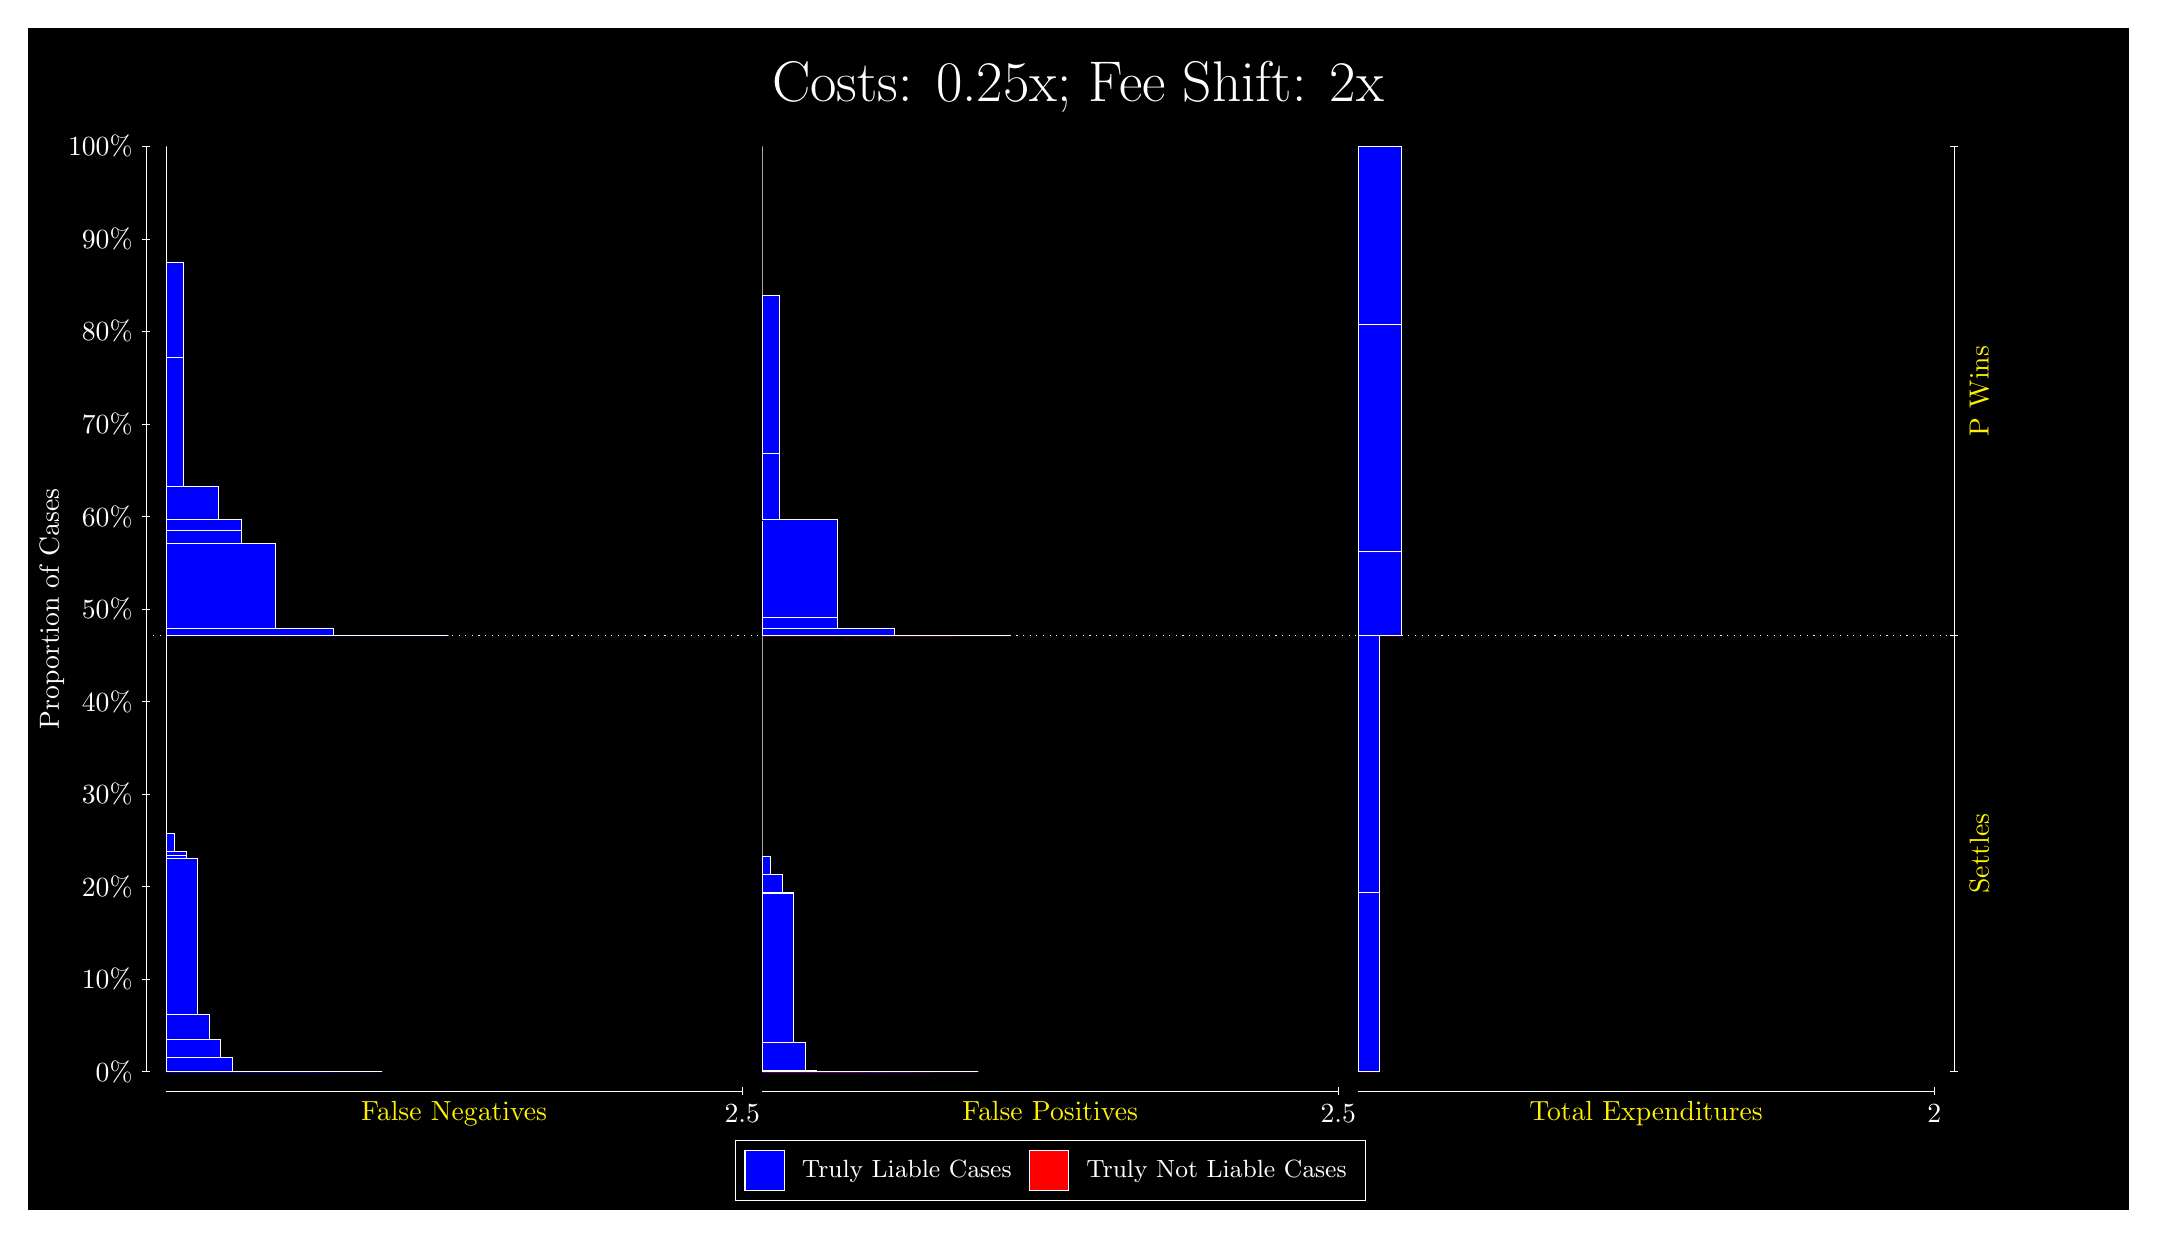
\begin{tikzpicture}
\draw[fill=black] (0,0) rectangle (26.667,15);
\draw[text=white] (0,13.5) rectangle (26.667,15) node[midway] {\huge Costs: 0.25x; Fee Shift: 2x};
\draw[white, very thin] (1.5,1.75) -- (1.5,13.5);
\node[rotate=90, text=white, anchor=center] at (0.3, 7.625) {Proportion of Cases};
\draw[white, very thin] (1.45,1.75) -- (1.55,1.75);
\node[text=white, anchor=east] at (1.45, 1.75) {0\%};
\draw[white, very thin] (1.45,2.925) -- (1.55,2.925);
\node[text=white, anchor=east] at (1.45, 2.925) {10\%};
\draw[white, very thin] (1.45,4.1) -- (1.55,4.1);
\node[text=white, anchor=east] at (1.45, 4.1) {20\%};
\draw[white, very thin] (1.45,5.275) -- (1.55,5.275);
\node[text=white, anchor=east] at (1.45, 5.275) {30\%};
\draw[white, very thin] (1.45,6.45) -- (1.55,6.45);
\node[text=white, anchor=east] at (1.45, 6.45) {40\%};
\draw[white, very thin] (1.45,7.625) -- (1.55,7.625);
\node[text=white, anchor=east] at (1.45, 7.625) {50\%};
\draw[white, very thin] (1.45,8.8) -- (1.55,8.8);
\node[text=white, anchor=east] at (1.45, 8.8) {60\%};
\draw[white, very thin] (1.45,9.975) -- (1.55,9.975);
\node[text=white, anchor=east] at (1.45, 9.975) {70\%};
\draw[white, very thin] (1.45,11.15) -- (1.55,11.15);
\node[text=white, anchor=east] at (1.45, 11.15) {80\%};
\draw[white, very thin] (1.45,12.325) -- (1.55,12.325);
\node[text=white, anchor=east] at (1.45, 12.325) {90\%};
\draw[white, very thin] (1.45,13.5) -- (1.55,13.5);
\node[text=white, anchor=east] at (1.45, 13.5) {100\%};

\draw[white, very thin] (24.457,1.75) -- (24.457,13.5);
\draw[white, very thin] (24.407,1.75) -- (24.507,1.75);
\node[anchor=west] at (24.407, 1.75) {};
\draw[white, very thin] (24.407,7.2867) -- (24.507,7.2867);
\node[anchor=west] at (24.407, 7.2867) {};
\draw[white, very thin] (24.407,13.5) -- (24.507,13.5);
\node[anchor=west] at (24.407, 13.5) {};

\draw[white, very thin, fill=blue] (1.75,1.75) rectangle (4.4946,1.75);
\draw[white, very thin, fill=blue] (1.75,1.75) rectangle (4.2018,1.75);
\draw[white, very thin, fill=blue] (1.75,1.75) rectangle (3.9091,1.75);
\draw[white, very thin, fill=blue] (1.75,1.75) rectangle (3.7627,1.75);
\draw[white, very thin, fill=blue] (1.75,1.75) rectangle (3.6163,1.75);
\draw[white, very thin, fill=blue] (1.75,1.75) rectangle (3.4699,1.75);
\draw[white, very thin, fill=blue] (1.75,1.75) rectangle (3.3236,1.7505);
\draw[white, very thin, fill=blue] (1.75,1.7505) rectangle (3.1772,1.7509);
\draw[white, very thin, fill=blue] (1.75,1.7509) rectangle (3.0308,1.7514);
\draw[white, very thin, fill=blue] (1.75,1.7514) rectangle (2.8844,1.7536);
\draw[white, very thin, fill=blue] (1.75,1.7536) rectangle (2.738,1.7576);
\draw[white, very thin, fill=blue] (1.75,1.7576) rectangle (2.5917,1.9287);
\draw[white, very thin, fill=blue] (1.75,1.9287) rectangle (2.4453,2.1593);
\draw[white, very thin, fill=blue] (1.75,2.1593) rectangle (2.2989,2.4711);
\draw[white, very thin, fill=blue] (1.75,2.4711) rectangle (2.1525,4.4566);
\draw[white, very thin, fill=blue] (1.75,4.4566) rectangle (2.0062,4.4952);
\draw[white, very thin, fill=blue] (1.75,4.4952) rectangle (2.0062,4.5483);
\draw[white, very thin, fill=blue] (1.75,4.5483) rectangle (1.8598,4.7802);
\draw[white, very thin, fill=red] (1.75,4.7802) rectangle (1.75,4.7802);
\draw[white, very thin, fill=blue] (1.75,4.7802) rectangle (1.75,7.2867);
\draw[white, very thin, fill=blue] (1.75,7.2867) rectangle (5.3362,7.2867);
\draw[white, very thin, fill=blue] (1.75,7.2867) rectangle (4.6044,7.2877);
\draw[white, very thin, fill=blue] (1.75,7.2877) rectangle (4.1652,7.2877);
\draw[white, very thin, fill=blue] (1.75,7.2877) rectangle (3.8725,7.3823);
\draw[white, very thin, fill=blue] (1.75,7.3823) rectangle (3.4333,7.3824);
\draw[white, very thin, fill=blue] (1.75,7.3824) rectangle (3.1406,8.4603);
\draw[white, very thin, fill=blue] (1.75,8.4603) rectangle (2.7015,8.6258);
\draw[white, very thin, fill=blue] (1.75,8.6258) rectangle (2.7015,8.7618);
\draw[white, very thin, fill=blue] (1.75,8.7618) rectangle (2.4087,9.1818);
\draw[white, very thin, fill=blue] (1.75,9.1818) rectangle (1.9696,10.819);
\draw[white, very thin, fill=blue] (1.75,10.819) rectangle (1.9696,12.027);
\draw[white, very thin, fill=red] (1.75,12.027) rectangle (1.75,12.027);
\draw[white, very thin, fill=blue] (1.75,12.027) rectangle (1.75,13.5);
\draw[white, very thin, fill=red] (9.3189,1.75) rectangle (12.063,1.75);
\draw[white, very thin, fill=blue] (9.3189,1.75) rectangle (12.063,1.75);
\draw[white, very thin, fill=red] (9.3189,1.75) rectangle (11.478,1.75);
\draw[white, very thin, fill=blue] (9.3189,1.75) rectangle (11.478,1.75);
\draw[white, very thin, fill=blue] (9.3189,1.75) rectangle (11.332,1.75);
\draw[white, very thin, fill=red] (9.3189,1.75) rectangle (11.185,1.75);
\draw[white, very thin, fill=blue] (9.3189,1.75) rectangle (11.185,1.75);
\draw[white, very thin, fill=red] (9.3189,1.75) rectangle (10.892,1.75);
\draw[white, very thin, fill=blue] (9.3189,1.75) rectangle (10.892,1.75);
\draw[white, very thin, fill=blue] (9.3189,1.75) rectangle (10.746,1.75);
\draw[white, very thin, fill=red] (9.3189,1.75) rectangle (10.6,1.75);
\draw[white, very thin, fill=blue] (9.3189,1.75) rectangle (10.6,1.7513);
\draw[white, very thin, fill=blue] (9.3189,1.7513) rectangle (10.453,1.7513);
\draw[white, very thin, fill=red] (9.3189,1.7513) rectangle (10.307,1.7513);
\draw[white, very thin, fill=blue] (9.3189,1.7513) rectangle (10.307,1.7522);
\draw[white, very thin, fill=blue] (9.3189,1.7522) rectangle (10.161,1.756);
\draw[white, very thin, fill=red] (9.3189,1.756) rectangle (10.014,1.756);
\draw[white, very thin, fill=blue] (9.3189,1.756) rectangle (10.014,1.7588);
\draw[white, very thin, fill=blue] (9.3189,1.7588) rectangle (10.014,1.7602);
\draw[white, very thin, fill=blue] (9.3189,1.7602) rectangle (9.8678,2.116);
\draw[white, very thin, fill=red] (9.3189,2.116) rectangle (9.7214,2.116);
\draw[white, very thin, fill=blue] (9.3189,2.116) rectangle (9.7214,4.0198);
\draw[white, very thin, fill=blue] (9.3189,4.0198) rectangle (9.7214,4.0203);
\draw[white, very thin, fill=blue] (9.3189,4.0203) rectangle (9.575,4.2565);
\draw[white, very thin, fill=blue] (9.3189,4.2565) rectangle (9.4287,4.4884);
\draw[white, very thin, fill=blue] (9.3189,4.4884) rectangle (9.3189,7.2867);
\draw[white, very thin, fill=red] (9.3189,7.2867) rectangle (12.466,7.2867);
\draw[white, very thin, fill=blue] (9.3189,7.2867) rectangle (12.466,7.2867);
\draw[white, very thin, fill=red] (9.3189,7.2867) rectangle (11.734,7.2867);
\draw[white, very thin, fill=blue] (9.3189,7.2867) rectangle (11.734,7.2877);
\draw[white, very thin, fill=red] (9.3189,7.2877) rectangle (11.002,7.2877);
\draw[white, very thin, fill=blue] (9.3189,7.2877) rectangle (11.002,7.3805);
\draw[white, very thin, fill=red] (9.3189,7.3805) rectangle (10.563,7.3805);
\draw[white, very thin, fill=blue] (9.3189,7.3805) rectangle (10.563,7.3805);
\draw[white, very thin, fill=red] (9.3189,7.3805) rectangle (10.27,7.3805);
\draw[white, very thin, fill=blue] (9.3189,7.3805) rectangle (10.27,7.5164);
\draw[white, very thin, fill=blue] (9.3189,7.5164) rectangle (10.27,8.7593);
\draw[white, very thin, fill=red] (9.3189,8.7593) rectangle (9.8312,8.7593);
\draw[white, very thin, fill=blue] (9.3189,8.7593) rectangle (9.8312,8.7598);
\draw[white, very thin, fill=blue] (9.3189,8.7598) rectangle (9.5384,9.6033);
\draw[white, very thin, fill=blue] (9.3189,9.6033) rectangle (9.5384,11.605);
\draw[white, very thin, fill=red] (9.3189,11.605) rectangle (9.3189,11.605);
\draw[white, very thin, fill=blue] (9.3189,11.605) rectangle (9.3189,13.5);
\draw[white, very thin, fill=red] (16.888,1.75) rectangle (17.162,1.75);
\draw[white, very thin, fill=blue] (16.888,1.75) rectangle (17.162,4.0235);
\draw[white, very thin, fill=red] (16.888,4.0235) rectangle (17.162,4.0235);
\draw[white, very thin, fill=blue] (16.888,4.0235) rectangle (17.162,7.2867);
\draw[white, very thin, fill=red] (16.888,7.2867) rectangle (17.437,7.2867);
\draw[white, very thin, fill=blue] (16.888,7.2867) rectangle (17.437,8.3519);
\draw[white, very thin, fill=red] (16.888,8.3519) rectangle (17.437,8.3519);
\draw[white, very thin, fill=blue] (16.888,8.3519) rectangle (17.437,11.237);
\draw[white, very thin, fill=red] (16.888,11.237) rectangle (17.437,11.237);
\draw[white, very thin, fill=blue] (16.888,11.237) rectangle (17.437,13.5);
\draw[white, dotted] (1.5,7.2867) -- (24.457,7.2867);
\draw[white, very thin] (1.75,1.5) -- (9.0689,1.5);
\node[text=yellow, anchor=north] at (5.4094, 1.5) {False Negatives};
\draw[white, very thin] (9.0689,1.45) -- (9.0689,1.55);
\node[text=white, anchor=north] at (9.0689, 1.45) {2.5};

\draw[white, very thin] (9.3189,1.5) -- (16.638,1.5);
\node[text=yellow, anchor=north] at (12.978, 1.5) {False Positives};
\draw[white, very thin] (16.638,1.45) -- (16.638,1.55);
\node[text=white, anchor=north] at (16.638, 1.45) {2.5};

\draw[white, very thin] (16.888,1.5) -- (24.207,1.5);
\node[text=yellow, anchor=north] at (20.547, 1.5) {Total Expenditures};
\draw[white, very thin] (24.207,1.45) -- (24.207,1.55);
\node[text=white, anchor=north] at (24.207, 1.45) {2};

\node[text=yellow, centered, rotate=90] at (24.777, 4.5183) {Settles};
\node[text=yellow, centered, rotate=90] at (24.777, 10.393) {P Wins};

\draw (12.978300999999998,1.5) node[draw=none] (baseCoordinate) {};
\begin{scope}[align=center]
        \matrix[scale=0.5, draw=white, below=0.5cm of baseCoordinate, nodes={draw}, column sep=0.1cm]{
            \node[rectangle, draw, minimum width=0.5cm, minimum height=0.5cm, fill=blue] {}; &
            \node[draw=none, font=\small, text=white] (B) {Truly Liable Cases}; &
            \node[rectangle, draw, minimum width=0.5cm, minimum height=0.5cm, fill=red] {}; &
            \node[draw=none, font=\small, text=white] (B) {Truly Not Liable Cases}; \\
            };
\end{scope}

\end{tikzpicture}
\end{document}